% --- Template for thesis / report with tktltiki2 class ---
%
% last updated 2013/02/15 for tkltiki2 v1.02

\documentclass[finnish]{tktltiki2}

  % tktltiki2 automatically loads babel, so you can simply
  % give the language parameter (e.g. finnish, swedish, english, british) as
  % a parameter for the class: \documentclass[finnish]{tktltiki2}.
  % The information on title and abstract is generated automatically depending on
  % the language, see below if you need to change any of these manually.
  %
  % Class options:
  % - grading                 -- Print labels for grading information on the front page.
  % - disablelastpagecounter  -- Disables the automatic generation of page number information
  %                              in the abstract. See also \numberofpagesinformation{} command below.
  %
  % The class also respects the following options of article class:
  %   10pt, 11pt, 12pt, final, draft, oneside, twoside,
  %   openright, openany, onecolumn, twocolumn, leqno, fleqn
  %
  % The default font size is 11pt. The paper size used is A4, other sizes are not supported.
  %
  % rubber: module pdftex

  % --- General packages ---

  \usepackage[utf8]{inputenc}
  \usepackage[T1]{fontenc}
  \usepackage{lmodern}
  \usepackage{microtype}
  \usepackage{amsfonts,amsmath,amssymb,amsthm,booktabs,color,enumitem,graphicx}
  \usepackage[pdftex,hidelinks]{hyperref}

  \graphicspath{{images/}}

  % Automaticall set the PDF metadata fields
  \makeatletter
  \AtBeginDocument{\hypersetup{pdftitle = {\@title}, pdfauthor = {\@author}}}
  \makeatother

  % --- Language-related settings ---
  %
  % these should be modified according to your language

  % babelbib for non-english bibliography using bibtex
  \usepackage[fixlanguage]{babelbib}
  \selectbiblanguage{finnish}

  % add bibliography to the table of contents
  \usepackage[nottoc]{tocbibind}
  % tocbibind renames the bibliography, use the following to change it back
  \settocbibname{Lähteet}

  % --- Theorem environment definitions ---

  \newtheorem{lau}{Lause}
  \newtheorem{lem}[lau]{Lemma}
  \newtheorem{kor}[lau]{Korollaari}

  \theoremstyle{definition}
  \newtheorem{maar}[lau]{Määritelmä}
  \newtheorem{ong}{Ongelma}
  \newtheorem{alg}[lau]{Algoritmi}
  \newtheorem{esim}[lau]{Esimerkki}

  \theoremstyle{remark}
  \newtheorem*{huom}{Huomautus}


  % --- tktltiki2 options ---
  %
  % The following commands define the information used to generate title and
  % abstract pages. The following entries should be always specified:

  \title{Konvoluutioneuroverkot}
  \author{Teemu Sarapisto}
  \date{\today}
  \level{Aine}
  \abstract{Viimeisen hieman yli kymmenen vuoden aikana voidaan sanoa keinotekoisten neuroverkkojen ja syväoppimisen tehneen läpimurron. Syväoppimisen voidaan katsoa syntyneen jo 40-luvulla, mutta laajamittaiseen sovelluskäyttöön se on tullut vasta viime vuosina, kun sekä riittävä määrä luokiteltua dataa, että riittävästi prosessointitehoa on tullut helposti saataville. Myös algoritmipuolella tapahtuneet edistykset ovat edesauttaneet läpimurtoa. Aikaisemmin koneoppimisen alalla haasteelliseksi osoittautuneissa sovelluskohteissa kuten kuvien sekä puheen sisällön tunnistamisessa keinotekoiset neuroverkot ovat osoittautuneet toistaiseksi ylivoimaisesti parhaiten toimiviksi ratkaisuiksi.}

  % The following can be used to specify keywords and classification of the paper:

  \keywords{avainsana 1, avainsana 2, avainsana 3}

  % classification according to ACM Computing Classification System (http://www.acm.org/about/class/)
  % This is probably mostly relevant for computer scientists
  % uncomment the following; contents of \classification will be printed under the abstract with a title
  % "ACM Computing Classification System (CCS):"
  % \classification{}

  % If the automatic page number counting is not working as desired in your case,
  % uncomment the following to manually set the number of pages displayed in the abstract page:
  %
  % \numberofpagesinformation{16 sivua + 10 sivua liitteissä}
  %
  % If you are not a computer scientist, you will want to uncomment the following by hand and specify
  % your department, faculty and subject by hand:
  %
  % \faculty{Matemaattis-luonnontieteellinen}
  % \department{Tietojenkäsittelytieteen laitos}
  % \subject{Tietojenkäsittelytiede}
  %
  % If you are not from the University of Helsinki, then you will most likely want to set these also:
  %
  % \university{Helsingin Yliopisto}
  % \universitylong{HELSINGIN YLIOPISTO --- HELSINGFORS UNIVERSITET --- UNIVERSITY OF HELSINKI} % displayed on the top of the abstract page
  % \city{Helsinki}
  %


  \begin{document}

  % --- Front matter ---

  \frontmatter      % roman page numbering for front matter

  \maketitle        % title page
  \makeabstract     % abstract page

  \tableofcontents  % table of contents

  % --- Main matter ---

  \mainmatter       % clear page, start arabic page numbering

  \section{Johdanto}
   Syväoppimisen historia ulottuu 1940-luvulle asti, jolloin kybernetiikan tutkimuksen myötä McCulloch ja Pitts kehittivät mukaansa nimetyn McCulloch-Pitts neuronin, tarkoituksenaan luoda matemaattinen malli jolla kuvailla biologista aivoissa tapahtuvaa oppimista. Heidän kehittelemällään lineaarisella mallilla oli mahdollista tunnistaa kahden syötekategorian välillä kummasta on kyse kategoriat määrittelevien painotuksien (weights) avulla, ihmisen joutuessa määrittelemään nämä painot.

  Vasta 1950-luvulla kehitettiin ensimmäinen malli joka pystyi oppimaan syötekategorioita kuvaavat painotukset niistä annettujen esimerkkien perusteella, niin kutsuttu perseptroni.

  Kiinnostuksen kybernetiikkaan hiivuttua 1960-luvun aikana, seuraavan kerran merkittävää kehitystä tapahtui 80-90-luvulla konnektionismin tuodessa neuroverkkomallit takaisin suosioon. Yksi tärkeimmistä näihin aikoihin tapahtuneista kehityksistä syväoppimisen kannalta oli, kun takaisinvirtausalgoritmin (backpropagation) keksittiin 1986 mahdollistavan monikerroksisten neuroverkkojen harjoittamisen verrattain tehokkaasti.

  90-luvun puolivälin jälkeen syväoppiminen eli jälleen hiljaiseloa vuoteen 2006 asti, jonka jälkeen se on ollut jatkuvasti pinnalla tähän päivään asti. Geoffrey Hinton osoitti tällöin syvien uskomusverkkojen (deep belief network) olevan harjoitettavissa tehokkaasti tasoittain ja muut tutkimusryhmät yleistivät tämän harjoitustavan muille syville keinotekoisille neuroverkoille. Näiden tutkimuksien myötä syväoppiminen terminä alkoi yleistyä, termin käytön tarkoituksena korostaa aikaisempaa syvempien verkkojen harjoitettavissa olemista.

  Lopullinen syväoppimisen läpimurto tapahtui vuonna 2012 kun suurimman kuvista objektien tunnistamisen kilpailun, ImageNet Large Scale Visual Recognition Challengen (ILSVRC), voitti ensimmäistä kertaa syvä (konvoluutio)neuroverkko. Voitto tapahtui myös huomattavalla erolla toisen sijan saavuttaneeseen sekä aikaisempien vuosien voittajiin. Tämän jälkeen kilpailun on joka vuosi voittanut syvä konvoluutioverkko, ja nykyään neuroverkot pärjäävät kyseisessä (varsin rajoitetussa) tunnistamistehtävässä ihmistä paremmin.

  Nykyään käytössä olevat ihmisille monimutkaisissakin tehtävissä pärjäävät oppimisalgoritmit ovat pääasiassa samoja kuin jo 80-luvulla käytössä olleet. Jonkin verran muutoksia silloisiin algoritmeihin on tehty syvien verkkorakenteiden harjoittamista helpottavina yksinkertaistuksina, mutta selkeästi suurin syy syväoppimisen tärkeäksi muuttumiseen vasta äskettäin on kuitenkin yhteiskunnan digitalisoitumisen myötä merkittävästi kasvanut helposti saatavilla olevan luokitellun datan määrä, sekä valtavasti kasvanut laskentakapasiteetti, jotka olivat edellytyksiä algoritmien kunnolliselle toiminnalle.

  Esimerkkinä tarvittavan harjoitusdatan määrästä konvoluutioneuroverkkojen harjoittamiseen kuvien luokittelua varten toimii yleensä tuhansia ellei jopa miljoonia kuvien sisällön perusteella etukäteen luokiteltuja kuvia. Esimerkiksi ILSVRC-kilpailun harjoitusdatana käytössä oleva ImageNet sisältää yli 14 miljoonaa luokiteltua kuvaa. (http://image-net.org/about-stats)

  Kuvien sisällön tunnistamisen lisäksi syväoppiminen on osoittautunut erittäin hyödylliseksi useissa haasteellisissa sovelluskohteissa, kuten puheen sisällön, liikennemerkkien luokittelun sekä jalankulkijoiden tunnistamisessa.

  %Tänä päivänä, vaikka neurotiedettä pidetäänkin tärkeänä inspiraation lähteenä syväoppimiselle, se ei kuitenkaan enää ole ensisijainen alaa eteenpäin vievä tekijä.

  \section{Neuroverkkojen rakenne}
  \subsection{Keinotekoinen neuroni}

    TODO: selkiytä kaavahommelia

    Biologisista vaikuttimistaan huolimatta keinotekoiset neuronit ovat käytännössä Kaavan \ref{eq:neuroni} muotoisia matemaattisia funktioita.

    \begin{equation}
      \label{eq:neuroni}
      \Sigma w_i x_i \mapsto f(\Sigma w_i x_i + b)
    \end{equation}

    Yleisessä muodossaan neuroni ottaa vastaan yhden tai useampia syötteitä $x_1$, $x_2$, ..., $x_n$, joista kullekin on asetettu jokin painoarvo $w_i$. Syötteiden ja painotuksien tulojen summa $\Sigma x_i w_i$ annetaan parametrina aktivaatiofunktiolle $f$ ja tämän funktion arvo toimii neuronin lopullisena ulostuloarvona.

    Toisinaan käytetään myös taipumusvakiota (bias) $b$, joka lisätään syötteiden ja painotuksien tulojen summaan.


    %You can think of the bias as a measure of how easy it is to get the perceptron to output a 1. Or to put it in more biological terms, the bias is a measure of how easy it is to get the perceptron to fire

    Ensimmäinen tällainen neuroni, perseptroni, kehitettiin 50-luvulla. Sen syötteet ja ulostuloarvot ovat binäärisiä ja aktivaatiofunktiona toimii Kaavan \ref{eq:perceptron} mukainen funktio.

    \begin{equation}
      \label{eq:perceptron}
      ulostuloarvo
      \begin{cases}
        0\; jos \; \Sigma x_i w_i + b \leq 0 \\
        1\; jos \; \Sigma x_i w_i + b > 0 \\
      \end{cases}
    \end{equation}

    Yksittäisen neuronin tasolla neuronien oppiminen tapahtuu syötteiden painotuksien ja taipumusarvon muuttumisen kautta. Perseptroneja käytettäessä törmätään kuitenkin usein ongelmaan, jossa yksi pieni muutos painotuksissa tai taipumusarvossa johtaa ulostuloarvon vaihtumiseen, joka saattaa aiheuttaa suuria muutoksia ulostuloarvoissa myös koko neuroverkon tasolla. Usein halutaan hienovaraisempia muutoksia ja tällöin käytetään neuroneita joiden syöte- ja paluuarvot voivat olla myös mitä vain reaalilukuja nollan ja yhden väliltä. Esimerkiksi yksi tällainen laajalti käytössä oleva neuroni on sigmoidinen neuroni, jonka aktivaatiofunktiona toimii sigmoidinen funktio.

  %kappaleessa 3 rojanista hyvää juttua \cite{Rojas96}

  %http://neuralnetworksanddeeplearning.com/chap1.html keksi parempi lähde
  % oliko varmasti 50-luvulla?

  \subsection{Keinotekoisten neuroverkkojen rakenne}

  \begin{figure}[h]
  \label{pic:neuralnet}
  \centering
  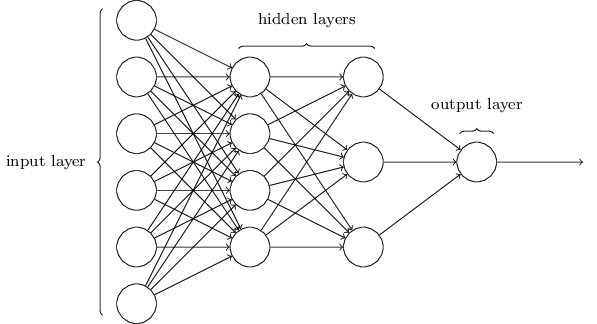
\includegraphics[scale=0.5]{basic-neuralnet}
  \caption{http://neuralnetworksanddeeplearning.com/chap1.html}
  \end{figure}

  Yksinkertaisimman verkkorakenteen omaavat eteenpäinsyöttävät neuroverkot muodostetaan tasoittain, jossa jokaisen verkon tason neuronit saavat syötteenään niitä edeltävän tason neuroneiden ulostuloarvot. Poikkeuksena ensimmäinen taso (kuvassa vasemmanpuoleisimpana), joihin verkon syöte koodataan. Esimerkiksi haluttaessa syöttää 64x64 kuva neuroverkolle, voidaan syötekerroksena käyttää 64x64 neuronin kerrosta, johon kuvan pikselien väriarvot koodataan.

  Vaikka syväoppimista voidaan harjoittaa myös muutoin kuin keinotekoisilla neuroverkoilla, neuroverkkojen tapauksessa termillä viitataan neuroverkkojen piilokerroksiin ja niiden määrään. Kasvattamalla neuroverkkotasojen sekä tasoissa olevien neuronien määrää neuroverkoilla voidaan mallintaa entistä monimutkaisempia funktioita.

  \section{Neuroverkkojen harjoittaminen}

  Neuroverkkojen on todistettu olevan universaaleja approksimaattoreita, eli voidaan taata, että mille tahansa funktiolle on löydettävissä neuroverkko, joka pystyy mallintamaan funktiota halutulla tarkkuudella, kunhan laskentaresursseja on riittävästi käytettävissä \cite{multilayer-feedforward-universal-approximators}. Neuroverkkojen harjoittamisen voidaan siis sanoa olevan neuroverkon tekemän virheen minimointia sen approksimoidessa jotakin funktiota.

  Tätä neuroverkon tekemän virheen määrää voidaan mitata virhefunktion (error function) avulla. Usein käytetään neliöllistä virhefunktiota:
    $$C(x) = \frac{1}{2} \sum_{i=1}^{N} \| y(x_i)-a(x_i) \|^2$$
  jossa $y(x_i)$ on neuroverkon tulos syötteellä $x_i$, $a(x_i)$ on harjoitusdatan $i$:s yksikkö, ja $N$ syötteiden määrä.


  \subsection{Gradienttimenetelmä ja takaisinvirtausalgoritmi}

  Takaisinvirtausalgoritmilla etsitään virhefunktion minimiä säätämällä painotuksia ja taipumusvakioita käyttäen gradienttimenetelmää (gradient descent).

  Gradienttimenetelmä on metodi joka toimii minkä tahansa derivoituvan funktion lokaalien minimien etsintään. Neuroverkkojen tapauksessa gradienttimenetelmän käytön edellytyksenä siis on, että neuronien aktivaatiofunktiot ovat jatkuvia funktioita, jolloin myös koko neuroverkon tuottamat arvot ja siten virhefunktio ovat jatkuvia. Gradientti kertoo mihin suuntaan funktion arvo laskee nopeimmin, joten kuljettaessa iteratiivisesti tähän suuntaan kunnes gradientti on tarpeeksi pieni, päädytään lähelle paikallista minimiä.

  Takaisinvirtausalgoritmi saa nimensä siitä, että eteenpäinsyötön jälkeen kuljetaan taaksepäin, ja lopulta solmulle x verkossa ollaan laskettu käytännössä derivaatat putkelle ja jotain.


  %tarvitseeko omaa otsikkoa, pitäisikö vain olla kappale takaisinvirtausalgoritmin otsikon alla?

  %batch gradient descent

  %Neuroverkon laskiessa ulostuloarvon jollekkin syötteelle, tapahtuu eteenpäinkulkeutumista (forward-propagation).

  Muuttamalla neuroverkon painoja ja taipumusvakioita suuntaan jonka gradientti osoittaa olevan negatiivinen voidaan minimoida virhefunktiota. Tätä toistetaan kunnes virhefunktio antaa riittävän pienen tuloksen. Jotta jokaista gradientin laskentakertaa varten ei tarvitsisi suorittaa takaisinvirtausalgoritmia syötedatan jokaista yksikköä kohden, voidaan käyttää stokastista gradientin laskeutumismenetelmää approksimointiin, joka yleensä tuottaa huomattavasti nopeammin hyviä tuloksia. TODO: Batch vs stochastic.

  Esittele syntaksi jolla tiettyyn verkon "solmuun" viitataan?

  Takaisinvirtausalgoritmi (back-propagation) (numeerinen menetelmä?) kertoo kuinka muutokset painoihin ja taipumusvakioihin muuttavat virhefunktion saamia arvoja. Näiden muutoksien perusteella voidaan laskea osittaisderivaatat painotuksille sekä taipumusvakioille virhefunktion suhteen. Osittaisderivaattojen avulla saadaan virhefunktiolle gradientti, ja gradientin laskeutumismenetelmällä voidaan minimoida virhefunktiota.

  %Jotta takaisinvirtausalgoritmia ei tarvitsisi ajaa jokaiselle harjoitusmateriaalin yksikölle, voidaan harjoitusmateriaalille laskea (tilastollisia arvoja?) keskiarvoja ja käyttää näitä keskiarvoja laskeutumismenetelmässä hyväksi. Ei välttämättä haluta ajaa takaisinvirtausalgoritmia uudestaan jokaiselle harjoitus"materiaalin" yksikölle. Voidaan ottaa niistä vain jotain keskiarvoja tms eli batching skjfdghsg



  \subsection{Ongelmia}

  Suuri haaste neuroverkkojen harjoittamisessa on ylisovitus (overfitting) jossa neuroverkon virhefunktion arvo on harjoitusdatalla saatu erittäin pieneksi, mutta uuden datan kanssa virhefunktio antaa suuria arvoja. Tällöin neuroverkon oppima malli vastaa harjoitusdataa liian tarkkaan, eikä enää suoriudu yleisestä tapauksesta toivotulla tavalla. Ylisovitusta korjaamaan on kehitetty metodeja kuten esimerkiksi neuroniyksikköjen pudotus (dropout) jossa harjoitusvaiheessa yksittäisiä neuroneita poistetaan satunnaisesti käytöstä, joka estää yksittäisiä neuroneita naapureineen erikoistumatta tiettyyn datan ominaisuuteen liian tarkasti.

  Neuroverkkojen harjoittamisessa olennaisessa osassa on myös verkon alkuperäisten painotuksien valitseminen sopivalla tavalla. Joissakin tapauksissa tämä tehdään vain valitsemalla painotuksille satunnaiset alkuarvot.

  \section{Konvoluutioneuroverkkojen rakenne}
  (TODO: ReLu)
  \subsection{Konvoluutiokerrokset}

  \begin{figure}[h]
  \label{pic:convolution}
  \centering
  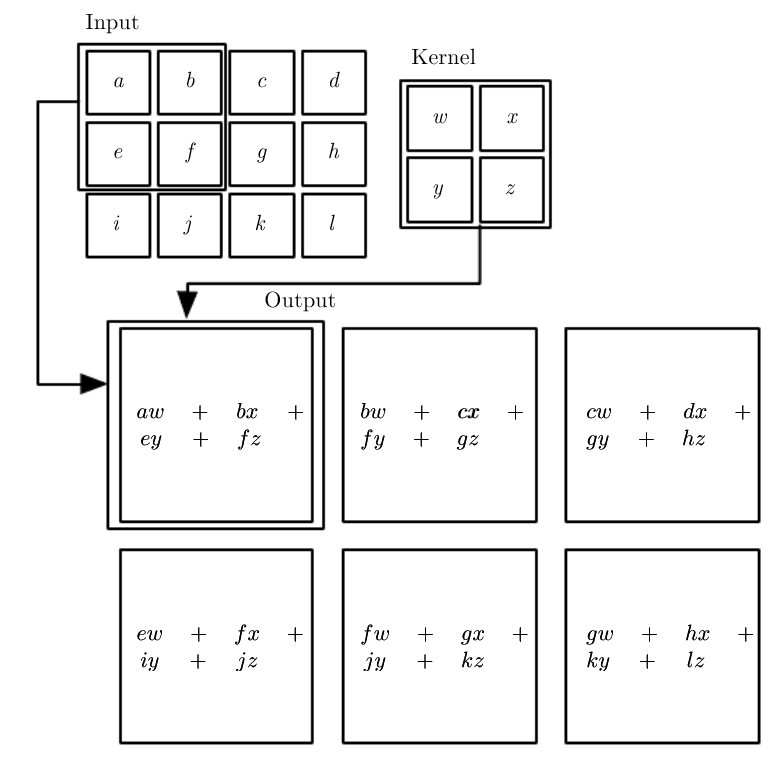
\includegraphics[scale=0.4]{convolution}
  \caption{http://www.deeplearningbook.org/contents/convnets.html}
  \end{figure}

  Konvoluutiokerroksissa neuronit saavat syötteenään vain osan syötekerroksensa ulostuloista. Tätä kutsutaan local receptive fieldsiksi. Esitettäessä konvoluutiokerrosten neuronien ulostuloarvot syötteidensä funktiona, tämä funktio on syötteiden ja painojen konvoluutio, mistä konvolutionaaliset neuroverkot ovatkin saaneet nimensä.

  (TODO: muotoile:) Vaikka vierekkäiset neuronikerrokset eivät ole täysin kytkettyjä, välillisesti muutaman kerroksen päässä olevat neuronit yleensä saavat syötteensä koko syötekerrokselta.

  Kuvan \ref{pic:convolution} mukaisesti mikäli tehdään vain "valid" konvoluutioita joissa ytimen täytyy olla täysin syötekuvan sisällä, konvoluutiokerroksella on vähemmän ulostuloja kuin sisääntuloja.

  \subsection{feature maps/detectors}
  Yhdessä konvoluutiokerroksessa on useita ominaisuuskarttoja :D (feature detectors)

  \subsection{shared weights}

  \subsection{pooling}
  Poolaus? funktio muuttaa verkon tietyn osan ulostulon verkon lähialueita kuvastavan yhteenvetävän tilastollisen arvon (summary statistic) mukaiseksi.
  \subsection{flattening}
  Konvoluutiokerrosten yhdistäminen täysin yhdistettyjen kerrosten kanssa

  \subsection{full connection}

  \section{Konvoluutioneuroverkkojen sovellukset}
  \subsection{Kuvien luokittelu}
  Tuloskerroksessa käytännössä todennäköisyysarvio luokittain











  % ------------------------------ References ------------------------------
  %
  % bibtex is used to generate the bibliography. The babplain style
  % will generate numeric references (e.g. [1]) appropriate for theoretical
  % computer science. If you need alphanumeric references (e.g [Tur90]), use
  %
  % \bibliographystyle{babalpha-lf}
  %
  % instead.

  \nocite{*}
  \bibliographystyle{babplain-lf}
  \bibliography{references}


  % --- Appendices ---

  % uncomment the following

  % \newpage
  % \appendix
  %
  % \section{Esimerkkiliite}

  \end{document}
